%https://www.gnu.org/software/emacs/manual/html_node/emacs/Fill-Commands.html
%https://academic.oup.com/journals/pages/authors/latex_files
%latexmk -pdf -pvc -auxdir=/Users/larshovdanmolden/Documents/Output/  article2_mancap.tex

\documentclass[review,fleqn]{elsarticle}\usepackage[]{graphicx}\usepackage[]{color}
% maxwidth is the original width if it is less than linewidth
% otherwise use linewidth (to make sure the graphics do not exceed the margin)
\makeatletter
\def\maxwidth{ %
  \ifdim\Gin@nat@width>\linewidth
    \linewidth
  \else
    \Gin@nat@width
  \fi
}
\makeatother

\definecolor{fgcolor}{rgb}{0.345, 0.345, 0.345}
\newcommand{\hlnum}[1]{\textcolor[rgb]{0.686,0.059,0.569}{#1}}%
\newcommand{\hlstr}[1]{\textcolor[rgb]{0.192,0.494,0.8}{#1}}%
\newcommand{\hlcom}[1]{\textcolor[rgb]{0.678,0.584,0.686}{\textit{#1}}}%
\newcommand{\hlopt}[1]{\textcolor[rgb]{0,0,0}{#1}}%
\newcommand{\hlstd}[1]{\textcolor[rgb]{0.345,0.345,0.345}{#1}}%
\newcommand{\hlkwa}[1]{\textcolor[rgb]{0.161,0.373,0.58}{\textbf{#1}}}%
\newcommand{\hlkwb}[1]{\textcolor[rgb]{0.69,0.353,0.396}{#1}}%
\newcommand{\hlkwc}[1]{\textcolor[rgb]{0.333,0.667,0.333}{#1}}%
\newcommand{\hlkwd}[1]{\textcolor[rgb]{0.737,0.353,0.396}{\textbf{#1}}}%
\let\hlipl\hlkwb

\usepackage{framed}
\makeatletter
\newenvironment{kframe}{%
 \def\at@end@of@kframe{}%
 \ifinner\ifhmode%
  \def\at@end@of@kframe{\end{minipage}}%
  \begin{minipage}{\columnwidth}%
 \fi\fi%
 \def\FrameCommand##1{\hskip\@totalleftmargin \hskip-\fboxsep
 \colorbox{shadecolor}{##1}\hskip-\fboxsep
     % There is no \\@totalrightmargin, so:
     \hskip-\linewidth \hskip-\@totalleftmargin \hskip\columnwidth}%
 \MakeFramed {\advance\hsize-\width
   \@totalleftmargin\z@ \linewidth\hsize
   \@setminipage}}%
 {\par\unskip\endMakeFramed%
 \at@end@of@kframe}
\makeatother

\definecolor{shadecolor}{rgb}{.97, .97, .97}
\definecolor{messagecolor}{rgb}{0, 0, 0}
\definecolor{warningcolor}{rgb}{1, 0, 1}
\definecolor{errorcolor}{rgb}{1, 0, 0}
\newenvironment{knitrout}{}{} % an empty environment to be redefined in TeX

\usepackage{alltt}
\usepackage[textsize=tiny,colorinlistoftodos]{todonotes}
\usepackage{subfig}
\usepackage{subcaption}





\usepackage{lineno,hyperref,float}
\usepackage{amsmath,natbib,bm}
\usepackage{geometry,array,setspace,lipsum,nccmath}
\usepackage{amsfonts}
\usepackage{booktabs}
\usepackage{siunitx}
\usepackage{rotating}
\usepackage{hypcap}
\usepackage{adjustbox}
\usepackage{pdflscape}
\setstretch{1.0}
\usepackage{color}
\usepackage{framed}
\usepackage{comment}
%\definecolor{shadecolor}{gray}{0.875}
\usepackage{caption}
%\captionsetup[table]{skip=8pt}
\usepackage{enumitem}
\usepackage{longtable}
% Table float box with bottom caption, box width adjusted to content
\usepackage{afterpage}
\usepackage{blindtext}
\usepackage{alltt}
\usepackage{graphicx}
\usepackage{graphics}
\usepackage{tikz}
\usepackage{tcolorbox}

\usetikzlibrary{shapes.geometric, arrows}
\usetikzlibrary{arrows.meta}
\usepackage{tikzscale}
\tikzset{every picture/.style={font issue=\footnotesize},
	font issue/.style={execute at begin picture={#1\selectfont}}
}


\renewcommand\labelitemi{--}
\tolerance=1600


\hypersetup{
  colorlinks=true,
  linkcolor=blue,    % color of internal links
  citecolor=blue,    % color of links to bibliography
  urlcolor=blue,     % color of external links
  allcolors=blue,
  bookmarksopen=true,
  pdfdisplaydoctitle=true
}
%\usepackage[doublespacing]{setspace}
%%\renewcommand\arraystretch{1.3}

\makeatletter
\@addtoreset{section}{part}
\makeatother
%\setcounter{secnumdepth}{0} % sections are level 1
\newcommand\T{\rule{0pt}{2.6ex}}       % Top strut
\newcommand\B{\rule[-1.2ex]{0pt}{0pt}} % Bottom strut
%\renewcommand{\familydefault}{\sfdefault}

\makeatletter
\renewcommand{\todo}[2][]{%
    \@todo[caption={#2}, #1]{\begin{spacing}{0.5}#2\end{spacing}}%
} 
\makeatother 

\usepackage{natbib}
%\bibpunct{(}{)}{;}{a}{,}{,}
%\usepackage{biblatex}
%\addbibresource{test}
\usepackage{tocloft}

%\usepackage{harvard}
\modulolinenumbers[5]

\journal{TBD}

%%APA style
\bibliographystyle{model5-names}\biboptions{authoryear}
%\specialcomment{answer}{\begin{shaded}}{\end{shaded}}

%% `Elsevier LaTeX' style
%\bibliographystyle{elsarticle-num}
%%%%%%%%%%%%%%%%%%%%%%%
\setlength\parindent{0pt}
\setlength{\parskip}{6pt}



%%\IfFileExists{upquote.sty}{\usepackage{upquote}}{}
\setlength{\mathindent}{0pt} %% NB MAYBEREMOVE BEFORE SUBMISSION


%%%% TURN OFF PAGE NUMBER FOR INCLUSION IN THESIS
%\pagenumbering{gobble}
%%%%%%%
\IfFileExists{upquote.sty}{\usepackage{upquote}}{}
\begin{document}

\begin{frontmatter}


\title{Dynamic capabilities and competitive advantage}
%\tnotetext[mytitlenote]{Fully documented templates are available in the elsarticle package on \href{http://www.ctan.org/tex-archive/macros/latex/contrib/elsarticle}{CTAN}.}

%% Group authors per affiliation:
%\author{Lars Hovdan Molden \fnref{myfootnote}}
%\address{Kongensgt 42, 7713 Steinkjer}
%\fntext[myfootnote]{Nord University Business School}

%% or include affiliations in footnotes:
%\author[mymainaddress,mysecondaryaddress]{Elsevier Inc}
%\ead[url]{www.elsevier.com}

%\author[mysecondaryaddress]{Global Customer Service\corref{mycorrespondingauthor}}
%\cortext[mycorrespondingauthor]{Corresponding author}
%\ead{support@elsevier.com}

%\address[mymainaddress]{1600 John F Kennedy Boulevard, Philadelphia}
%\address[mysecondaryaddress]{360 Park Avenue South, New York}

\begin{abstract}
 We find that DC as routines to shape routines is most prevelant under moderate dynamism,
whereas DC as routines to capture resources in factor markets are more prevelant under
dynamic environments.

\end{abstract}

\begin{keyword}
\texttt{Dynamic Capabilities, Deliberate Learning, Dynamics }
\end{keyword}

\end{frontmatter}

%\linenumbers


\doublespacing


\section{Introduction}

The relationship between dynamic capabilities and competitive advantage has been one of
great contention in the extant literature \citep{Peteraf2013,Ambrosini2009}. From this
debate a richer understanding of how different dynamic capabilities (or functional forms
of them) work differently to change different types of firm resources
\citep{Helfat2015a,Teece2007,Ambrosini2009a} with implications for competitive advantage
\citep{Peteraf2013}.  has emerged.  work dDC offers a theory of how firms achieve
competitive advantage over time. Yet the DC theory suffers from contradictory claims about
competitive advantage as its outcome. On the one hand a stream of contributions argue that
DC will lead to competitive advantage because it operates by changing operational
capabilities in face of change and hence create strategic change (ref helfat). In this
view these changes result in complex and path dependent processes that will be
idiosyncratic to the firm and hard to imitate. Consequently, they can lead to competitive
advantage.

A contrary stream of literature argues that changes of operational capabilities over time
takes the form of routines and converges towards best practice (ref EM). Such best
practices are simpler and more observable routines that are both imitable and easy to
copy. Such firm resources are then not idiosyncratic and can consequently not be the
source of competitive advantage. 

The way DC work differnelty throug changing two sets of operational capabilities = complex
and path dependent processes based capabilities, and simple rules/based routines. 

These contradictory positions have been thoroughly discussed in earlier work (see
\cite{Peteraf2013} for a review). On the one hand DC takes the form of simple rules
shaping underlying routines. On the other hand they take the form of complex processes.  

Regarding the action and the object ofthe action, simple rules are more likely to be
involved in developing something new in response to new opportunities, while complex
rou- tines are more concerned with changing existing resources and capabilities.

In a recent "state of the art" literature review on dynamic capabilities
\cite{Schilke2018} state that much of the attention and interest surrounding the theory is
that it offer a route to competitive advantage which they argue is "the virtual Holy Grail
of strategic management" (p. 393). And indeed a considerable body of the extant literature
concerns itself with exactly this path to competitive advantage (refs from
shcilke). Still, a discourse regarding the contingencies of the dynamic
capabilities-competitive advantage (DC-CA) nexus (?) has panned out in the literature,
most notably coined "the elephant in the room" \citep{Peteraf2013}: Under which conditions
will dynamic capabilities lead to competitive advantage?

\cite{Peteraf2013} argue that the seminal papers in the dynamic capabilities theory
tradition (\cite{Teece1997} and \cite{Eisenhardt2000}) differ considerably in their view
of to what extent the DC-CA nexus exist and under what conditions it is functional. A key
tenant of this discourse is related to the level of routinization and the ability to
satisfy the VRIO condition \citep{Barney1991a} of the resource-based view
\citep{Peteraf2013}.

In this paper we aim to contribute to dissecting the elephant by asking how does the DC-CA
nexus differ between firms and what determines these differences?

We do this by exploring two paths from dynamic capabilities to competitive advantage: the
\emph{evolutionary path} and the \emph{market path}. The former is thoroughly described
and explored in the literature (refs) and stems from the core idea of the dynamic
capabilities theorizing. In this path dynamic capabilities work to change the operating
routines of the firm and hence contributing to it's competitive advantage. We argue that
this path is more suited for less dynamic environments because of its path dependent
functioning.

The \emph{market path} works not through shaping operational capabilities and routines,
but by enabling the firm to act in factor markets for new capabilities and
resources. Hence, it is less path dependent and can be more rapidly
deployed. Consequently, it is more prevalent in dynamic environments.

This paper contributes to the extant literature on the link between dynamic capabilities
and competitive advantage in three ways. First, provides an empirical test to the
drive-train model of \cite{DiStefano2014} on how dynamic capabilities can operate both
quickly and with high frequency more directly on the strategic direction of the firm by
acting in factor markets for important resources, and also more slowly through the
evolutionary path of changing operational capabilities. Second, by conceptually clarifying
the different paths to competitive advantage by linking it closely to the role of
capability evolution and the VRIO condition. Finally, we.........

CLARIFIES THE ROLE OF THE ENVIRONMENT AND MEDIATIONS HAPPENING

%% How does dynamic capabilities lead to competitive advantage?
%% Dynamic capabilities are proposed to confer a competitive advantage by adding unique value to the firm through systematic change, which enhances operational efficiency and enables increased alignment with the environment (Di Stefano et al., 2014; Peteraf et al., 2013)

%% Not all organizations possess them (Collis, 1996); their path dependencies, intangibility, complexity, and organizational specificity make them hard to imitate (Gibson & Birkinshaw, 2004; Helfat & Winter, 2011); and few other means allow organizations to purposefully change on a continuous basis (Day & Wensley, 1988; Helfat et al., 2007).

%% Consistent with the theoretical positions of Eisenhardt and Martin (2000), Helfat and Peteraf (2003), Zahra et al. (2006), and Zott (2003), among others, these researchers have argued that dynamic capabilities’ immediate purpose is to change the resource base, and that this change in the resource base, in turn, explains performance variations. According to this argument, resource changes serve as mediators through which dynamic capabilities affect performance. We


%% One of the major unresolved issues in dynamic capabilities theory is to what extent and
%% how competitive advantage is the ultimate outcome of dynamic capabilities. This very idea
%% has


%% This paper asks two questions: to what extent does a direct lnk between DC and CA exist,
%% and what determines variations in the role of mediation between them?

%% The idea that Dc impacts CA is uncontroversial (not). Little is known about how this
%% happens. The theory holds that this happens through xreating extending and modifying the
%% resource base. YEt, the change in firm capabilities can themselves lead to CA due to their
%% evlutionary nature.

%% Variations in the share of mediation stems from variation sin the environment. When envdyn
%% is high firms need to act faster and hence tends to choose strategies including resource
%% orchestration buying in factor markets cause it tkes more time to develop OR.

%% In less dynamism the role of OR increases and leads to a significant proportion of CA
%% stemming throhg the mediating effect of OR

%% There is ongoing interest in (dynamic) capabilities and how they influence firm
%% performance \citep{Fainshmidt2016a,Teece2014}. Indeed, \emph{dynamic capabilities} (DC),
%% and its front runner, the resource-based view \citep{Barney2001,Helfat2007}, is now
%% considered one of the major theories in strategic management
%% \citep{Schilke2018}. Arguably, the key reason is that this theory clearly articulates how
%% firms can alter their operating routines through dynamic capabilities. Thus, a key
%% ingredient in this theory is that DCs can alter firms operating routines, with subsequent
%% performance implications.


We demonstrate that two paths indeed do exist and that their relative importance varies
with the degree of environmental dynamism facing the firm.

\section{Hypotheses}\label{sec:hyp}

%% We can use the drive train to determine hwo DC works differently under different levels of
%% dynamism. It is not that DC does not work under stable conditions as EM claims. Is only
%% that the effect runs stringer through the evolutionary path. Whereas the market path is
%% stringer under higher dynamism


One contentious issue surrounding the DC theory is the extent to which differing views on
the nature of dynamic capabilities \citep{Peteraf2013} as well as their outcome. One
strand of contributions sees DC as routines that are simple in nature and more as best
practices to consider (EM). Thus, dynamic capabilities are more like behavioral patterns
and less idiosyncratic to the firm and will consequently not be able to satisfy the VRIO
condition for competitive advantage to emerge. Dynamic capabilities as such routines are
short lived, unstable and “substitutable” (EM: 1110) thus violating a key VRIN condition,
and they are more “more homogeneous (..) than is usually assumed” (EM: 1116). However, the
simplicity of simple rules also makes them faster do deploy and put in motion, albeit
potentially unstable. To the extent dynamic capabilities manifest themselves as simple
rules they cannot alone create competitive advantage, but could very well generate
strategic change by facilitating acquisition of resources in factor markets. One example
is the role of post-acquisition routines where routines to identify and deal with
acquisition partners are a source of generating strategic change (Eisenhardt and Sull
2001, ref). Another example is (see refs from Schilke 2018). The functioning of this
expression of dynamic capabilities are more latent and hence mainly observable ex
post. Hence we can see this as direct route to competitive advantage as this expression of
dynamic capabilities work directly in the factor market in capturing resources
needed for strategic change. We coin this direct connection as the \emph{market path}.

On the other hand, a stream of contributions see dynamic capabilities as evolutionary and
more complex routines (ref) or processes (ref) set to change underlying capabilities in
the face of changing conditions (TPS). This notion stems from evolutionary economics
\citep{Winter2003,Nelson1982} and the behavioral theory of the firm \citep{Cyert1963}
holding that path dependency and complex processes for changing underlying operating
routines are a source of competitive advantage for the firm. Along this indirect path
change is gradual and running through changes in underlying routines. We coin this the
\emph{evolutionary path}.

These paths from dynamic capabilities to competitive advantage are different expressions
of dynamic capabilities with different mediums of intermediation. The \emph{market path}
works in the market and his hence not typically altering lower order capabilities and
resources in the firm directly, but rather acquiring new ones. The source of competitive
advantage along this path stems from the interaction with the other, \emph{evolutionary
  path} in a dynamic bundle \citep{Peteraf2013}. Such interactions create a bundle of
capabilities and routines that are socially complex and hard to imitate
\citep[p. 320]{DiStefano2014}. Moreover, the interactions between the two paths of dynamic
capabilities is separable with respect to what intermediation exist. Consequently,
separate paths exist albeit a part of a dynamic bundle.

\cite{DiStefano2014} propose an integrated framework where simple routines and more
complex processes could contribute simultanously to the firms outcome, specifically its
competitive advantage. In this framework, coined the "organizational drivetrain" the
authors envision the movement of an organization as set in motion by a drivetrain system
not unlike that of a bicycle.

Building on the notion of an organizational drivetrain we argue that dynamic capabilities
can indeed impact the organizational movement or change through two distinct but
interconnected mechanisms (i.e. the crank set and the rear shifter). The two mechanisms
consitutting the drivetrain is consistent with our notion of \emph{evolutionary path} and the \emph{market path}. The
evolutionary path is instigated by more complex processes setting in motiong a chance in
the lower order (operational) routines \cite{Collis1994,Winter2003}. In the drivetrain
metaphor this path corresponds to change stemming from the front crank set of thich there
are fewer gears, but with larger impact. This path is slower
and yields a more idiosyncratic set of organizational routines which is very much in line
with the idea put forth in the seminal founding papers \citep{Teece1997,Winter2003}.

Seeing the bike rider and her efforts to handle the levers of control (i.e. the gear
shifter) as the dynamic capability, and consider it not only as a management effort, but
that of the organization as a whole. The process of changing front gears are more profound
(i.e. evolutionary) and costly, and it is for larger and slower strategic
changes. Operating with simple routines in factor markets, however, is quicker and the
rider does this on a more frequent basis with less effort.

H1: Dynamic capabilities works to create competitive advantage through two distinctly
different paths.

\subsection{The two paths of dynamic capabilities}
The objective of strategic change is to enhance a firm’s competitive advantage
(ref). Doing so over time makes for the evolutionary fitness of the firm
\citep{Helfat2007}. When firms are developing capabilities for strategic change through
creating, extending and modifying the resource base this means making decisions to develop
operational routines. Such routines can in turn stem from an inherent learning process
evolutionary distinct to the firm. Operating routines can thus lead to competitive
advantage because of their evolutionary character \citep{Nelson1982,Winter2003}. To the
extent operating routines stems from idiosyncratic evolutionary process of individual
firms rather than being the result of investments in factor markets, they can satisfy the
VRIO condition and thus be a source of competitive advantage. In such instances, dynamic
capabilities work through operating routines in creating competitive advantage. This
indirect impact on competitive advantage is very much at the core of the DC literature
(ref). Firms with high dynamic capabilities will be able to better change operating
routines to facilitate strategic change in response to changing conditions facing the
firm. Dynamic capabilities then creates VRIO operating routines and hence competitive
advantage. When this happens, firms changes their operating routines in a evolutionary
making operating routines themselves OR itself satisfies the VRIO condition.

\emph{H2: Dynamic capabilities has an indirect effect on competitive advantage through
  changing the operating routines of the firm.}

On the other hand, resources and capabilities can to a certain extent be captured in
factor markets through investment decisions (ref) or through alliances (ref) or M\&A
activates (ref). By acquiring resources through investments, the operating routines of the
firms may not be directly affected. When these acquisitions happen as a response to
systematic resource orchestration (ref), i.e. reshaping the resource mix to obtain
coordinated resource deployments \citep{Kor2005,Pan2006}, they would indeed have potential
performance implications for the firm. Moreover, when this process of resource acquisition
process of DC develops a way to acquire and mix resource for the purpose of adapting to
change, the resources themselves would not necessarily satisfy the VRIO condition. The way
in which this happens may be much harder to imitate due to the complexities such routines
exhibit. Although resources themselves exhibit clear equifinality in their impact on
competitive advantage, combined with the simple routines of the orchestration
(i.e. dynamic capabilities), the sum would likely satisfy the VRIO condition. This is
especially true if routines are deployed rapidly in changing market conditions. In other
words, there are several ways in which resources can be orchestrated to generate CA,
whereas improved OR will always mean improved competitiveness et ceteris paribus. In such
instances DC itself can lead to CA directly.

\emph{H3: Dynamic capabilities has a direct effect on competitive advantage through the
  process of resource orchestration and acquisition of resources in factor markets.}

In other words, we would expect DC to have both a direct and an indirect impact on CA. The
indirect impact stems from the \emph{evolutionary path} of complex processes, whereas the
direct impact stems from the \emph{market path}.  Although both the direct and the
indirect path stems from DC creating, extending and modifying the resource base (OR or
factor market resources), the difference in the path’s stems from to what extent the
mediating construct alone can by itself satisfy the VRIO condition. Operating routines
can, due to their evolutionary nature, in turn shaped by DC, achieve CA
\citep{Collis1994,Winter2003}. Factor market resources and market acquired capabilities
and best practices can not \citep{Eisenhardt2000,Peteraf2013}, but in conjuncture with the
routines of acting in factor markets as well as the speed of deployment, the sum of
dynamic capabilities and factor market action would lead to competitive advantage.

However, the interlinkages between simple routines (the market path) and the coplex
processes (the evolutionary path) would vary with the environment.

\subsection{Interplay under environmental dynamism}

\cite{DiStefano2014} note that "even if specific simple rules are unstable and ephemeral,
the system as a whole is not" and that the "real source of sustainable competitive ad- vantage for an enterprise is the difficulty of imitating and substituting for the entire dynamic bundle that the system represents" (p.sss).

But the interlinkages between the parts of the system (the evolutionary- and the market
path), are likely to vary with the environmental dynamism. Under moderatly dynamism
dynamic capabilities takes the form of best pracitces (e.g. aquisition targeting) and is
less important than under more dynamic environments. However, albeit best practices, the
way they are implemented in the factor markets are still idiosyncratic. And taken into
conjunction with the routinzed process of changing underlying routines, VRIO will very
likely emerge under more stable conditions. It is not that the market/direct expression
of dynamic capabilities are not present in stable environments, rather it is less pronounced and the indirect
mediated effect (evolutionary path) is more important. In other words, it is not neither
nor, but degrees of importance.

Moreover, in high velocity environments the role of the evolutionary path tends to
weaken as such path-dependent changes occur slower compared to the market path. From the
market path with its simple routines we can argue that creation of "new knowledge” to
“allow for emergent adaptation” (EM, p. 1116) is the consequence. Consequently, the market
path is stronger and more prevalent under higher levels of environmental dynamism.

\emph{H4: Dynamic capabilities works relatively stronger through the market path in highly
dynamic environments.}


\begin{figure}
  \centering
  \captionsetup{width=0.5\linewidth}
  \includegraphics[width=0.5\linewidth]{./figure/fig2.png}
  \captionof{figure}{Dynamic capabilities direct and indirect paths to competitive advantage determined by the VRIO condition}
  \label{fig:fig2}
\end{figure}

Figure \ref{fig:fig2} illustrates the two proposed paths through which DC affect
competitive advantage. The main take away from this is that dynamic capabilities can
affect CA through changing operational routines that by themselves can satisfy the VRIO
condition by means of their evolutionary nature. Thus, we hypothesize that operating
routines mediates the relationship between dynamic capabilities and competitive advantage
the evolutionary path. Conversely, the same dynamic capabilities enable the firm to
identify resources and capabilities in factor markets that are less idiosyncratic and
often takes the shape of best practices that are definitely imitable and thus bot VRIO. In
such instances, the VRIO condition is satisfied by the DC itself through its complex
process of orchestrating and mixing resources – the market path.


\section{Data and methods}

To test the relationships between dynamic capabilities and competitive advantage we need a
proper metric of both. We also benefit vastly from studying the same firms over time.  The
lack of h longitudinal studies to investigate dynamics over time and control for path
dependency of organizational routines has been noted as permanent limitation for moving
the DC literature forward empirically and theoretically \cite{Schilke2018}.

We collected survey data from R\&D active firms in Norway at two points in time
($T_1=2005$ and $T_2=2014$). The population was all businesses registered to a scheme for
tax deduction of R\&D costs (called SkatteFUNN). As all enterprises which are eligible for
taxation could register their R\&D activities to receive a tax refund, the registered
enterprises include close to all enterprises which are involved in such activities at the
time of our study.

All firms that registered R\&D activities during May to December 2005 were approached
totaling in all 1721 firms. A web-based questionnaire was developed containing the
measures of the key constructs of this paper. A link to the questionnaire was e-mailed to
the firms within a month after they registered R\&D activities. The initial mailing was
followed by two e-mail reminders. Of the firms approached, 1199 (70 \%) returned filled-in
questionnaires. The 1199 companies that filled out the questionnaire were contacted again
9 years later. The majority of firms were contacted in spring/summer 2014. All received a
web-based questionnaire containing the same measures of the focal constructs of this
paper. 283 of the firms returned filled-in questionnaire.

All the firms in the sample was identifiable by means of the official firm
identifier. This enabled us to attach financial data from the annual accounts of the firms
despite none of the firms in the sample being publicly traded companies. We obtained the
financial accounts from the National Firm Registry (BRREG) for all years between 2007 and
2014 (prior to 2007 was not accessible through our database).

\subsection{Variable construction}

The focal constructs of this paper are dynamic capabilities, operational routines and
competitive advantage. These are all operationalized using the survey data described
above. Table 1 below describes the items used to operationalize the focal constructs and
their internal validity in forming an additive index (Cronbach´s alpha). The results show
that our key constructs can be represented by the items in the survey.


There are no established measurement models of dynamic capabilities
\citep{McKelvie2009,Schilke2018}. Therefore this study builds on a mixture of qualitative
case study methodology, literature review and statistical techniques to develop and refine
measures of DCs. First, exploratory qualitative interviews, using a semistructured
interview guide, were conducted with management representatives from 10 R\&D/innovative
firms. The aim of the interviews was to get an overview of each firm's innovation and
development processes, in particular the processes related to its dynamic capabilities and
the management of its resources. Themes raised in the interviews were about network,
co-operation with external R\&D-institutions, learning in the firm, adaptation and changes
in the firm. We interviewed SMEs and larger firms, and the industries varied from
high-tech and ICT to publishing.  Based on the interviews and an extensive literature
review, statements identified as descriptions of dynamic capabilities and resources were
developed and included in a questionnaire.

Second, the informants from the 10 firms were subsequently asked to take part in a pretest
of the questionnaire, including the preliminary items developed to measure dynamic
capabilities and resources, by responding to the questionnaire and giving comments on the
individual questions. This was followed up by a telephone call to the interviewees where
they were asked to report their views on the various questions/items.

Third, the face validity of the items was further examined by pre-testing the measurements
among experts. Researchers with knowledge of business strategy within firms were asked to
evaluate the questionnaire. Based on the results from the pilot study, the items were
adjusted and refined.

Although we recognize at the outset that the concept of dynamic capabilities and their
underlying resource components are very challenging to research in a systematic and
econometric fashion \citep{McKelvie2009}, we follow the argument in the
literature that more empirical work is necessary to test and refine the dynamic
capabilities concept and how it is related to the evolutionary economic theory
\citep{Arend2009,McKelvie2009} \todo{Rosenblom, 2000; Verona and Ravasi, 2003;}.  It
is in this spirit that the research reported in this paper has been undertaken.

Items measuring DC and OCs were developed as statements for which the respondents were
asked to indicate to what extent each statement fitted a description of their business. We
adopted one-sided seven point Likert scale where: 1 = strongly disagree and 7 = strongly
agree. We built on prior studies where items measuring OCs have been measured relative to
competitors \citep{McKelvie2009}.



  \providecommand{\huxb}[2]{\arrayrulecolor[RGB]{#1}\global\arrayrulewidth=#2pt}
  \providecommand{\huxvb}[2]{\color[RGB]{#1}\vrule width #2pt}
  \providecommand{\huxtpad}[1]{\rule{0pt}{\baselineskip+#1}}
  \providecommand{\huxbpad}[1]{\rule[-#1]{0pt}{#1}}

\begin{table}[h]
\centering
\begin{threeparttable}
\begin{tabularx}{0.9\textwidth}{p{0.18\textwidth} p{0.18\textwidth} p{0.18\textwidth} p{0.18\textwidth} p{0.18\textwidth}}


\hhline{}
\arrayrulecolor{black}

\multicolumn{1}{!{\huxvb{0, 0, 0}{0}}l!{\huxvb{0, 0, 0}{0}}}{\huxtpad{6pt}\raggedright \textbf{Factor}\huxbpad{6pt}} &
\multicolumn{1}{r!{\huxvb{0, 0, 0}{0}}}{\huxtpad{6pt}\raggedleft \textbf{Items}\huxbpad{6pt}} &
\multicolumn{1}{r!{\huxvb{0, 0, 0}{0}}}{\huxtpad{6pt}\raggedleft \textbf{Loading}\huxbpad{6pt}} &
\multicolumn{1}{r!{\huxvb{0, 0, 0}{0}}}{\huxtpad{6pt}\raggedleft \textbf{Alpha}\huxbpad{6pt}} &
\multicolumn{1}{r!{\huxvb{0, 0, 0}{0}}}{\huxtpad{6pt}\raggedleft \textbf{CI}\huxbpad{6pt}} \tabularnewline[-0.5pt]


\hhline{>{\huxb{0, 0, 0}{0.7}}->{\huxb{0, 0, 0}{0.7}}->{\huxb{0, 0, 0}{0.7}}->{\huxb{0, 0, 0}{0.7}}->{\huxb{0, 0, 0}{0.7}}-}
\arrayrulecolor{black}

\multicolumn{1}{!{\huxvb{0, 0, 0}{0}}l!{\huxvb{0, 0, 0}{0}}}{\huxtpad{6pt}\raggedright $CA$\huxbpad{6pt}} &
\multicolumn{1}{r!{\huxvb{0, 0, 0}{0}}}{\huxtpad{6pt}\raggedleft CA^1\huxbpad{6pt}} &
\multicolumn{1}{r!{\huxvb{0, 0, 0}{0}}}{\huxtpad{6pt}\raggedleft 0.86\huxbpad{6pt}} &
\multicolumn{1}{r!{\huxvb{0, 0, 0}{0}}}{\huxtpad{6pt}\raggedleft 0.83\huxbpad{6pt}} &
\multicolumn{1}{r!{\huxvb{0, 0, 0}{0}}}{\huxtpad{6pt}\raggedleft 0.90\huxbpad{6pt}} \tabularnewline[-0.5pt]


\hhline{}
\arrayrulecolor{black}

\multicolumn{1}{!{\huxvb{0, 0, 0}{0}}l!{\huxvb{0, 0, 0}{0}}}{\huxtpad{6pt}\raggedright \huxbpad{6pt}} &
\multicolumn{1}{r!{\huxvb{0, 0, 0}{0}}}{\huxtpad{6pt}\raggedleft CA^2\huxbpad{6pt}} &
\multicolumn{1}{r!{\huxvb{0, 0, 0}{0}}}{\huxtpad{6pt}\raggedleft 0.88\huxbpad{6pt}} &
\multicolumn{1}{r!{\huxvb{0, 0, 0}{0}}}{\huxtpad{6pt}\raggedleft ~~~\huxbpad{6pt}} &
\multicolumn{1}{r!{\huxvb{0, 0, 0}{0}}}{\huxtpad{6pt}\raggedleft ~~~\huxbpad{6pt}} \tabularnewline[-0.5pt]


\hhline{}
\arrayrulecolor{black}

\multicolumn{1}{!{\huxvb{0, 0, 0}{0}}l!{\huxvb{0, 0, 0}{0}}}{\huxtpad{6pt}\raggedright \huxbpad{6pt}} &
\multicolumn{1}{r!{\huxvb{0, 0, 0}{0}}}{\huxtpad{6pt}\raggedleft CA^3\huxbpad{6pt}} &
\multicolumn{1}{r!{\huxvb{0, 0, 0}{0}}}{\huxtpad{6pt}\raggedleft 0.85\huxbpad{6pt}} &
\multicolumn{1}{r!{\huxvb{0, 0, 0}{0}}}{\huxtpad{6pt}\raggedleft ~~~\huxbpad{6pt}} &
\multicolumn{1}{r!{\huxvb{0, 0, 0}{0}}}{\huxtpad{6pt}\raggedleft ~~~\huxbpad{6pt}} \tabularnewline[-0.5pt]


\hhline{>{\huxb{0, 0, 0}{0.2}}->{\huxb{0, 0, 0}{0.2}}->{\huxb{0, 0, 0}{0.2}}->{\huxb{0, 0, 0}{0.2}}->{\huxb{0, 0, 0}{0.2}}-}
\arrayrulecolor{black}

\multicolumn{1}{!{\huxvb{0, 0, 0}{0}}l!{\huxvb{0, 0, 0}{0}}}{\huxtpad{6pt}\raggedright $CA_t$\huxbpad{6pt}} &
\multicolumn{1}{r!{\huxvb{0, 0, 0}{0}}}{\huxtpad{6pt}\raggedleft CA_{t-1}^1\huxbpad{6pt}} &
\multicolumn{1}{r!{\huxvb{0, 0, 0}{0}}}{\huxtpad{6pt}\raggedleft 0.88\huxbpad{6pt}} &
\multicolumn{1}{r!{\huxvb{0, 0, 0}{0}}}{\huxtpad{6pt}\raggedleft 0.79\huxbpad{6pt}} &
\multicolumn{1}{r!{\huxvb{0, 0, 0}{0}}}{\huxtpad{6pt}\raggedleft 0.88\huxbpad{6pt}} \tabularnewline[-0.5pt]


\hhline{}
\arrayrulecolor{black}

\multicolumn{1}{!{\huxvb{0, 0, 0}{0}}l!{\huxvb{0, 0, 0}{0}}}{\huxtpad{6pt}\raggedright \huxbpad{6pt}} &
\multicolumn{1}{r!{\huxvb{0, 0, 0}{0}}}{\huxtpad{6pt}\raggedleft CA_{t-1}^2\huxbpad{6pt}} &
\multicolumn{1}{r!{\huxvb{0, 0, 0}{0}}}{\huxtpad{6pt}\raggedleft 0.80\huxbpad{6pt}} &
\multicolumn{1}{r!{\huxvb{0, 0, 0}{0}}}{\huxtpad{6pt}\raggedleft ~~~\huxbpad{6pt}} &
\multicolumn{1}{r!{\huxvb{0, 0, 0}{0}}}{\huxtpad{6pt}\raggedleft ~~~\huxbpad{6pt}} \tabularnewline[-0.5pt]


\hhline{}
\arrayrulecolor{black}

\multicolumn{1}{!{\huxvb{0, 0, 0}{0}}l!{\huxvb{0, 0, 0}{0}}}{\huxtpad{6pt}\raggedright \huxbpad{6pt}} &
\multicolumn{1}{r!{\huxvb{0, 0, 0}{0}}}{\huxtpad{6pt}\raggedleft CA_{t-1}^3\huxbpad{6pt}} &
\multicolumn{1}{r!{\huxvb{0, 0, 0}{0}}}{\huxtpad{6pt}\raggedleft 0.84\huxbpad{6pt}} &
\multicolumn{1}{r!{\huxvb{0, 0, 0}{0}}}{\huxtpad{6pt}\raggedleft ~~~\huxbpad{6pt}} &
\multicolumn{1}{r!{\huxvb{0, 0, 0}{0}}}{\huxtpad{6pt}\raggedleft ~~~\huxbpad{6pt}} \tabularnewline[-0.5pt]


\hhline{>{\huxb{0, 0, 0}{0.2}}->{\huxb{0, 0, 0}{0.2}}->{\huxb{0, 0, 0}{0.2}}->{\huxb{0, 0, 0}{0.2}}->{\huxb{0, 0, 0}{0.2}}-}
\arrayrulecolor{black}

\multicolumn{1}{!{\huxvb{0, 0, 0}{0}}l!{\huxvb{0, 0, 0}{0}}}{\huxtpad{6pt}\raggedright $DC_P$\huxbpad{6pt}} &
\multicolumn{1}{r!{\huxvb{0, 0, 0}{0}}}{\huxtpad{6pt}\raggedleft DC_P^1\huxbpad{6pt}} &
\multicolumn{1}{r!{\huxvb{0, 0, 0}{0}}}{\huxtpad{6pt}\raggedleft 0.71\huxbpad{6pt}} &
\multicolumn{1}{r!{\huxvb{0, 0, 0}{0}}}{\huxtpad{6pt}\raggedleft 0.82\huxbpad{6pt}} &
\multicolumn{1}{r!{\huxvb{0, 0, 0}{0}}}{\huxtpad{6pt}\raggedleft 0.88\huxbpad{6pt}} \tabularnewline[-0.5pt]


\hhline{}
\arrayrulecolor{black}

\multicolumn{1}{!{\huxvb{0, 0, 0}{0}}l!{\huxvb{0, 0, 0}{0}}}{\huxtpad{6pt}\raggedright \huxbpad{6pt}} &
\multicolumn{1}{r!{\huxvb{0, 0, 0}{0}}}{\huxtpad{6pt}\raggedleft DC_P^2\huxbpad{6pt}} &
\multicolumn{1}{r!{\huxvb{0, 0, 0}{0}}}{\huxtpad{6pt}\raggedleft 0.83\huxbpad{6pt}} &
\multicolumn{1}{r!{\huxvb{0, 0, 0}{0}}}{\huxtpad{6pt}\raggedleft ~~~\huxbpad{6pt}} &
\multicolumn{1}{r!{\huxvb{0, 0, 0}{0}}}{\huxtpad{6pt}\raggedleft ~~~\huxbpad{6pt}} \tabularnewline[-0.5pt]


\hhline{}
\arrayrulecolor{black}

\multicolumn{1}{!{\huxvb{0, 0, 0}{0}}l!{\huxvb{0, 0, 0}{0}}}{\huxtpad{6pt}\raggedright \huxbpad{6pt}} &
\multicolumn{1}{r!{\huxvb{0, 0, 0}{0}}}{\huxtpad{6pt}\raggedleft DC_P^3\huxbpad{6pt}} &
\multicolumn{1}{r!{\huxvb{0, 0, 0}{0}}}{\huxtpad{6pt}\raggedleft 0.70\huxbpad{6pt}} &
\multicolumn{1}{r!{\huxvb{0, 0, 0}{0}}}{\huxtpad{6pt}\raggedleft ~~~\huxbpad{6pt}} &
\multicolumn{1}{r!{\huxvb{0, 0, 0}{0}}}{\huxtpad{6pt}\raggedleft ~~~\huxbpad{6pt}} \tabularnewline[-0.5pt]


\hhline{}
\arrayrulecolor{black}

\multicolumn{1}{!{\huxvb{0, 0, 0}{0}}l!{\huxvb{0, 0, 0}{0}}}{\huxtpad{6pt}\raggedright \huxbpad{6pt}} &
\multicolumn{1}{r!{\huxvb{0, 0, 0}{0}}}{\huxtpad{6pt}\raggedleft DC_P^4\huxbpad{6pt}} &
\multicolumn{1}{r!{\huxvb{0, 0, 0}{0}}}{\huxtpad{6pt}\raggedleft 0.77\huxbpad{6pt}} &
\multicolumn{1}{r!{\huxvb{0, 0, 0}{0}}}{\huxtpad{6pt}\raggedleft ~~~\huxbpad{6pt}} &
\multicolumn{1}{r!{\huxvb{0, 0, 0}{0}}}{\huxtpad{6pt}\raggedleft ~~~\huxbpad{6pt}} \tabularnewline[-0.5pt]


\hhline{}
\arrayrulecolor{black}

\multicolumn{1}{!{\huxvb{0, 0, 0}{0}}l!{\huxvb{0, 0, 0}{0}}}{\huxtpad{6pt}\raggedright \huxbpad{6pt}} &
\multicolumn{1}{r!{\huxvb{0, 0, 0}{0}}}{\huxtpad{6pt}\raggedleft DC_P^5\huxbpad{6pt}} &
\multicolumn{1}{r!{\huxvb{0, 0, 0}{0}}}{\huxtpad{6pt}\raggedleft 0.82\huxbpad{6pt}} &
\multicolumn{1}{r!{\huxvb{0, 0, 0}{0}}}{\huxtpad{6pt}\raggedleft ~~~\huxbpad{6pt}} &
\multicolumn{1}{r!{\huxvb{0, 0, 0}{0}}}{\huxtpad{6pt}\raggedleft ~~~\huxbpad{6pt}} \tabularnewline[-0.5pt]


\hhline{>{\huxb{0, 0, 0}{0.2}}->{\huxb{0, 0, 0}{0.2}}->{\huxb{0, 0, 0}{0.2}}->{\huxb{0, 0, 0}{0.2}}->{\huxb{0, 0, 0}{0.2}}-}
\arrayrulecolor{black}

\multicolumn{1}{!{\huxvb{0, 0, 0}{0}}l!{\huxvb{0, 0, 0}{0}}}{\huxtpad{6pt}\raggedright $DC_X$\huxbpad{6pt}} &
\multicolumn{1}{r!{\huxvb{0, 0, 0}{0}}}{\huxtpad{6pt}\raggedleft DC_X^1\huxbpad{6pt}} &
\multicolumn{1}{r!{\huxvb{0, 0, 0}{0}}}{\huxtpad{6pt}\raggedleft 0.83\huxbpad{6pt}} &
\multicolumn{1}{r!{\huxvb{0, 0, 0}{0}}}{\huxtpad{6pt}\raggedleft 0.74\huxbpad{6pt}} &
\multicolumn{1}{r!{\huxvb{0, 0, 0}{0}}}{\huxtpad{6pt}\raggedleft 0.84\huxbpad{6pt}} \tabularnewline[-0.5pt]


\hhline{}
\arrayrulecolor{black}

\multicolumn{1}{!{\huxvb{0, 0, 0}{0}}l!{\huxvb{0, 0, 0}{0}}}{\huxtpad{6pt}\raggedright \huxbpad{6pt}} &
\multicolumn{1}{r!{\huxvb{0, 0, 0}{0}}}{\huxtpad{6pt}\raggedleft DC_X^2\huxbpad{6pt}} &
\multicolumn{1}{r!{\huxvb{0, 0, 0}{0}}}{\huxtpad{6pt}\raggedleft 0.72\huxbpad{6pt}} &
\multicolumn{1}{r!{\huxvb{0, 0, 0}{0}}}{\huxtpad{6pt}\raggedleft ~~~\huxbpad{6pt}} &
\multicolumn{1}{r!{\huxvb{0, 0, 0}{0}}}{\huxtpad{6pt}\raggedleft ~~~\huxbpad{6pt}} \tabularnewline[-0.5pt]


\hhline{}
\arrayrulecolor{black}

\multicolumn{1}{!{\huxvb{0, 0, 0}{0}}l!{\huxvb{0, 0, 0}{0}}}{\huxtpad{6pt}\raggedright \huxbpad{6pt}} &
\multicolumn{1}{r!{\huxvb{0, 0, 0}{0}}}{\huxtpad{6pt}\raggedleft DC_X^3\huxbpad{6pt}} &
\multicolumn{1}{r!{\huxvb{0, 0, 0}{0}}}{\huxtpad{6pt}\raggedleft 0.85\huxbpad{6pt}} &
\multicolumn{1}{r!{\huxvb{0, 0, 0}{0}}}{\huxtpad{6pt}\raggedleft ~~~\huxbpad{6pt}} &
\multicolumn{1}{r!{\huxvb{0, 0, 0}{0}}}{\huxtpad{6pt}\raggedleft ~~~\huxbpad{6pt}} \tabularnewline[-0.5pt]


\hhline{>{\huxb{0, 0, 0}{0.2}}->{\huxb{0, 0, 0}{0.2}}->{\huxb{0, 0, 0}{0.2}}->{\huxb{0, 0, 0}{0.2}}->{\huxb{0, 0, 0}{0.2}}-}
\arrayrulecolor{black}

\multicolumn{1}{!{\huxvb{0, 0, 0}{0}}l!{\huxvb{0, 0, 0}{0}}}{\huxtpad{6pt}\raggedright $P$\huxbpad{6pt}} &
\multicolumn{1}{r!{\huxvb{0, 0, 0}{0}}}{\huxtpad{6pt}\raggedleft P^1\huxbpad{6pt}} &
\multicolumn{1}{r!{\huxvb{0, 0, 0}{0}}}{\huxtpad{6pt}\raggedleft 0.71\huxbpad{6pt}} &
\multicolumn{1}{r!{\huxvb{0, 0, 0}{0}}}{\huxtpad{6pt}\raggedleft 0.70\huxbpad{6pt}} &
\multicolumn{1}{r!{\huxvb{0, 0, 0}{0}}}{\huxtpad{6pt}\raggedleft 0.84\huxbpad{6pt}} \tabularnewline[-0.5pt]


\hhline{}
\arrayrulecolor{black}

\multicolumn{1}{!{\huxvb{0, 0, 0}{0}}l!{\huxvb{0, 0, 0}{0}}}{\huxtpad{6pt}\raggedright \huxbpad{6pt}} &
\multicolumn{1}{r!{\huxvb{0, 0, 0}{0}}}{\huxtpad{6pt}\raggedleft P^2\huxbpad{6pt}} &
\multicolumn{1}{r!{\huxvb{0, 0, 0}{0}}}{\huxtpad{6pt}\raggedleft 0.82\huxbpad{6pt}} &
\multicolumn{1}{r!{\huxvb{0, 0, 0}{0}}}{\huxtpad{6pt}\raggedleft ~~~\huxbpad{6pt}} &
\multicolumn{1}{r!{\huxvb{0, 0, 0}{0}}}{\huxtpad{6pt}\raggedleft ~~~\huxbpad{6pt}} \tabularnewline[-0.5pt]


\hhline{}
\arrayrulecolor{black}

\multicolumn{1}{!{\huxvb{0, 0, 0}{0}}l!{\huxvb{0, 0, 0}{0}}}{\huxtpad{6pt}\raggedright \huxbpad{6pt}} &
\multicolumn{1}{r!{\huxvb{0, 0, 0}{0}}}{\huxtpad{6pt}\raggedleft P^3\huxbpad{6pt}} &
\multicolumn{1}{r!{\huxvb{0, 0, 0}{0}}}{\huxtpad{6pt}\raggedleft 0.85\huxbpad{6pt}} &
\multicolumn{1}{r!{\huxvb{0, 0, 0}{0}}}{\huxtpad{6pt}\raggedleft ~~~\huxbpad{6pt}} &
\multicolumn{1}{r!{\huxvb{0, 0, 0}{0}}}{\huxtpad{6pt}\raggedleft ~~~\huxbpad{6pt}} \tabularnewline[-0.5pt]


\hhline{>{\huxb{0, 0, 0}{0.2}}->{\huxb{0, 0, 0}{0.2}}->{\huxb{0, 0, 0}{0.2}}->{\huxb{0, 0, 0}{0.2}}->{\huxb{0, 0, 0}{0.2}}-}
\arrayrulecolor{black}

\multicolumn{1}{!{\huxvb{0, 0, 0}{0}}l!{\huxvb{0, 0, 0}{0}}}{\huxtpad{6pt}\raggedright $R$\huxbpad{6pt}} &
\multicolumn{1}{r!{\huxvb{0, 0, 0}{0}}}{\huxtpad{6pt}\raggedleft R^1\huxbpad{6pt}} &
\multicolumn{1}{r!{\huxvb{0, 0, 0}{0}}}{\huxtpad{6pt}\raggedleft 0.91\huxbpad{6pt}} &
\multicolumn{1}{r!{\huxvb{0, 0, 0}{0}}}{\huxtpad{6pt}\raggedleft 0.94\huxbpad{6pt}} &
\multicolumn{1}{r!{\huxvb{0, 0, 0}{0}}}{\huxtpad{6pt}\raggedleft 0.96\huxbpad{6pt}} \tabularnewline[-0.5pt]


\hhline{}
\arrayrulecolor{black}

\multicolumn{1}{!{\huxvb{0, 0, 0}{0}}l!{\huxvb{0, 0, 0}{0}}}{\huxtpad{6pt}\raggedright \huxbpad{6pt}} &
\multicolumn{1}{r!{\huxvb{0, 0, 0}{0}}}{\huxtpad{6pt}\raggedleft R^2\huxbpad{6pt}} &
\multicolumn{1}{r!{\huxvb{0, 0, 0}{0}}}{\huxtpad{6pt}\raggedleft 0.94\huxbpad{6pt}} &
\multicolumn{1}{r!{\huxvb{0, 0, 0}{0}}}{\huxtpad{6pt}\raggedleft ~~~\huxbpad{6pt}} &
\multicolumn{1}{r!{\huxvb{0, 0, 0}{0}}}{\huxtpad{6pt}\raggedleft ~~~\huxbpad{6pt}} \tabularnewline[-0.5pt]


\hhline{}
\arrayrulecolor{black}

\multicolumn{1}{!{\huxvb{0, 0, 0}{0}}l!{\huxvb{0, 0, 0}{0}}}{\huxtpad{6pt}\raggedright \huxbpad{6pt}} &
\multicolumn{1}{r!{\huxvb{0, 0, 0}{0}}}{\huxtpad{6pt}\raggedleft R^3\huxbpad{6pt}} &
\multicolumn{1}{r!{\huxvb{0, 0, 0}{0}}}{\huxtpad{6pt}\raggedleft 0.96\huxbpad{6pt}} &
\multicolumn{1}{r!{\huxvb{0, 0, 0}{0}}}{\huxtpad{6pt}\raggedleft ~~~\huxbpad{6pt}} &
\multicolumn{1}{r!{\huxvb{0, 0, 0}{0}}}{\huxtpad{6pt}\raggedleft ~~~\huxbpad{6pt}} \tabularnewline[-0.5pt]


\hhline{>{\huxb{0, 0, 0}{0.2}}->{\huxb{0, 0, 0}{0.2}}->{\huxb{0, 0, 0}{0.2}}->{\huxb{0, 0, 0}{0.2}}->{\huxb{0, 0, 0}{0.2}}-}
\arrayrulecolor{black}
\end{tabularx}\end{threeparttable}


\end{table}



\subsection{Control variables}

We add a set of control variables expected to explain parts of the variation in our focal
constructs. From the survey we add firm size, firm age, the level of dynamism facing the
firm. Size is the reported number of employees in the firm at $T_2$, and age is the number of
years since establishment. Dynamism is captured by asking a number of questions about the
competitive environment facing the firm. A full list of items and their internal validity
(0.75) is available in appendix 1111.

To partly remedy the problem of common method bias, we add controls of financial data from
the firm´s profit and loss statements, and balance sheet. Specifically, we add the natural
logarithm of the assets and debt of the firm to capture the leverage (debt risk) of the
firm, as well as the capital intensity.

One core critique of the dynamic capabilities literature is that it simply is a response
to the firm being a good firm \citep{Arend2009}. This tautology makes it hard to
distinguish the direction of the effects the performance implications of dynamic
capabilities. Simply put both firm performance and dynamic capabilities can be due to some
unobserved factor of the firm simply being a “good firm”. In such cases we would simply
regress one on the other and get positive results without the exact mechanism being
pointed out. To partly control for this we add a proxy for the quality of the firm as a
control variable. In this paper we use the profit margin of the firm as this type of
control. It is not perfect as profit margins can be due to many factors outside our model,
but it serves to control for parts of the possible cofounding factors of firm quality.

\subsection{Estimation and empirical model}

To test our hypotheses, we run a sequential linear regression with heteroskedastic robust
standard errors. We test the mediation hypotheses within this framework using a causal
mediation \citep{Baron1986,MacKinnon2008} with quasi-Bayesian confidence intervals and
over a million simulations \citep{Imai2010}.

In addition we estimate mediating models and test formally for mediation using the Baron
\& Kenny method \citep{Baron1986,MacKinnon2008}. We estimate two mediating model to test
if OR mediates the effect of DC on CA, and if DC mediates the effect of DL on OR,
respectively.

\section{Results}
The focal variables of our study is presented with pairwise correlation, mean and standard
deviation in table \ref{tab:desc}.It is worth noting that the mean value of OR and DC is
declining over time suggesting that the average firm experience a negative development in
core resources. The ability of the firms in our sample to generate CA is somewhat
unchanged over the sample period. We also observe a certain correlation in the development
in DC over time suggesting that prior period DC is a strong predictor of future
DC. Furthermore, we see a strong correlation between DL and DC which indicates that these
two constructs are indeed related.


\begin{figure}[ht] \label{ fig7} 
  \begin{minipage}[b]{0.5\linewidth}
    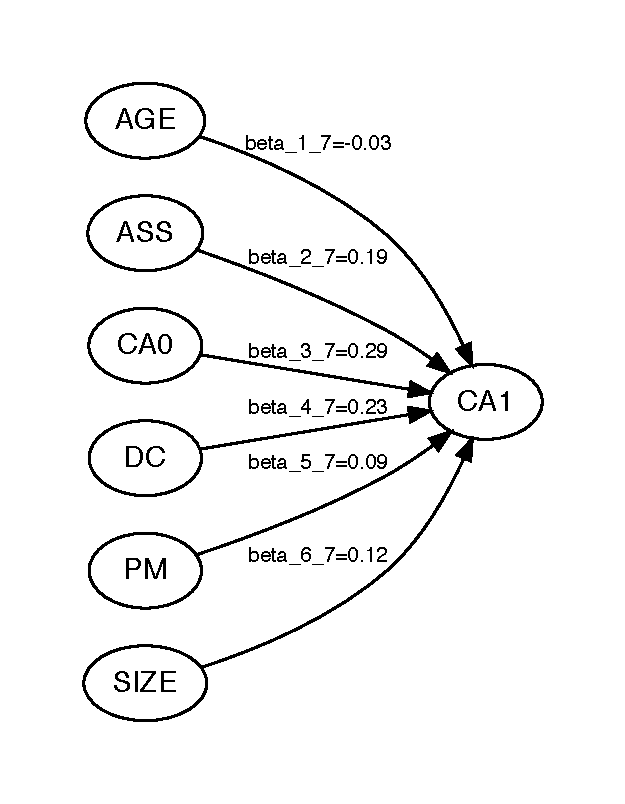
\includegraphics[width=.99\linewidth]{full.pdf} 
    \caption{Full model} 
  \end{minipage} 
  \begin{minipage}[b]{0.5\linewidth}
    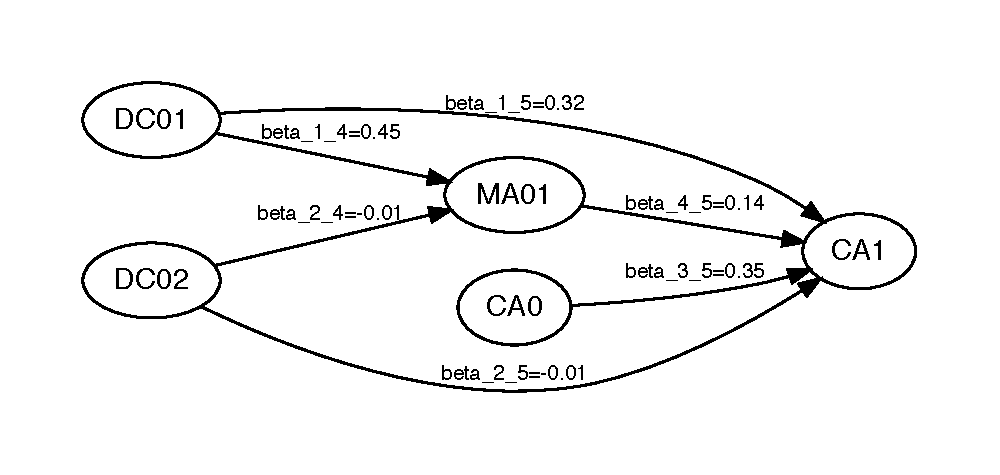
\includegraphics[width=.99\linewidth]{ma.pdf} 
    \caption{Routine mediation} 
  \end{minipage} 
  \begin{minipage}[b]{0.5\linewidth}
    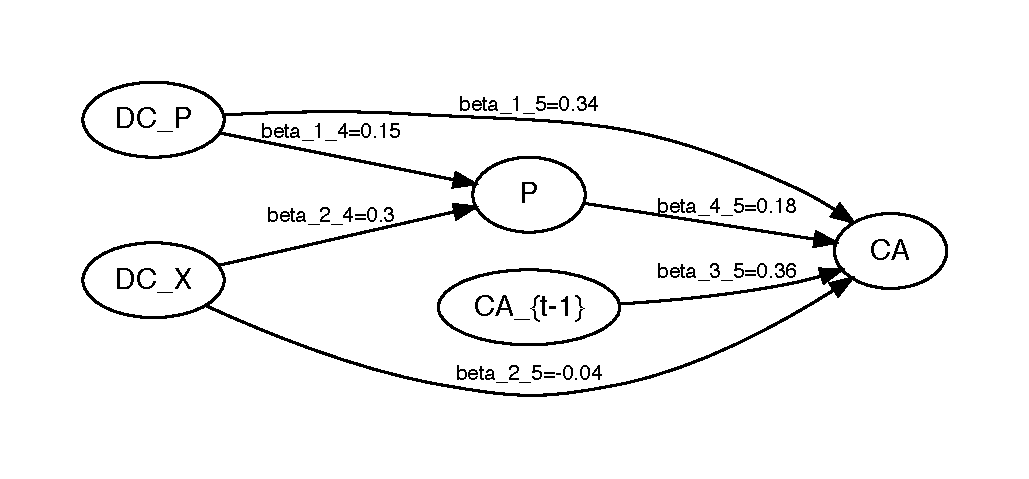
\includegraphics[width=.99\linewidth]{or.pdf} 
    \caption{Process mediation} 
  \end{minipage}
  \hfill
  \begin{minipage}[b]{0.5\linewidth}
    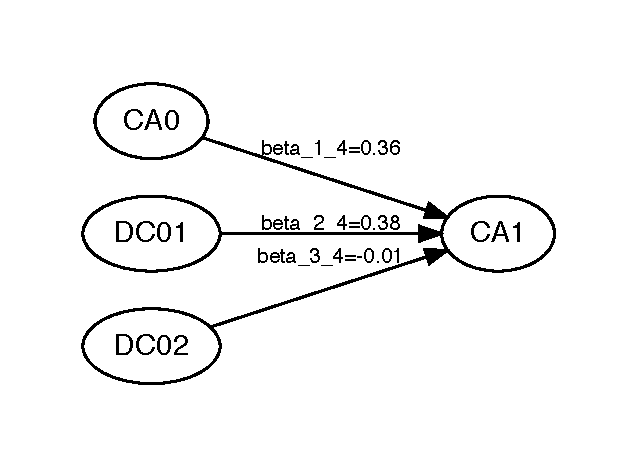
\includegraphics[width=.99\linewidth]{dir.pdf} 
    \caption{Direct model} 
  \end{minipage} 
\end{figure}


\begin{figure}
     \centering
  \caption{Structural model of full estimation - PLS-SEM}
  \begin{tikzpicture}
   \centering
   \tikzstyle{mynode}=[circle,draw, ultra thin, draw=black, fill=white, minimum size=17mm,inner sep=0pt, align=center]
        
   \node[mynode] (dc1){$DC_P$};
   \node[mynode,below of=dc1, yshift=-2cm] (dc2){$DC_X$};
   \node[mynode,right of=dc1, xshift=3cm] (or){$P$};
   \node[mynode,right of=dc2, xshift=3cm] (ma){$R$};
   \node[mynode,right of=ma, xshift=3cm, yshift=1.5cm] (ca){$CA$};
   
   
   \draw[-latex] (dc1.east) -- node[text width=0.5cm,font=\footnotesize, above=2pt,align=left,
   fill=white] {$0.129^{*}$} (or.west);

   \draw[-latex] (dc2.east) -- node[text width=0.5cm,font=\footnotesize, above=2pt, align=left,
   fill=white] {$-0.091^{}$} (ma.west);

   \draw[-latex] (dc1.south east) -- node[text width=0.5cm,font=\footnotesize,  above=2pt,
   align=left, fill=white,sloped, near end] {$0.496^{***}$} (ma.north west);

   \draw[-latex] (dc2.north east) -- node[text width=0.5cm,font=\footnotesize, above=2pt,align=left,
   fill=white,sloped, near end]{$0.343^{***}$} (or.south west);

    \draw[-latex] (or.east) -- node[text width=0.5cm,font=\footnotesize, align=left,above=2pt,
   fill=white,sloped]{$0.185^{***}$} (ca.north west);

   \draw[-latex] (ma.east) -- node[text width=0.5cm,font=\footnotesize, below=2pt,
   fill=white,sloped]{$0.123^{**}$} (ca.south west);

   \draw[-latex] (dc1.north)[bend left] to node[text width=0.5cm,font=\footnotesize, above=2pt,align=center,
   fill=white]{$0.299^{***}$}(ca.north);

   \draw[-latex] (dc2.south)[bend right] to node[text width=0.5cm,font=\footnotesize,below=2pt, align=left,
   fill=white]{$-0.066^{}$} (ca.south);
    
 
\end{tikzpicture}

\end{figure}

\begin{table}
\begin{center}
\script size
\begin{tabular}{lcccc}

\hline \\[-2pt]
 & \multicolumn{4}{c}{{\bf Models:}} \\  \cline{2-5} \\[-3pt] 
 & \emph{Direct} & \emph{Process} & \emph{Routines} & \emph{Full}\\
 & (1) & (2) & (3) & (4)\\
\hline
 &  &  &  & \\
\(CA_{t-1} \rightarrow CA\) & 0.364 & 0.361 & 0.351 & 0.343\\
 & (7.19) & (6.49) & (6.33) & (6.27)\\[3pt]
 &  &  &  & \\
\(DC_P \rightarrow CA\) & 0.378 & 0.342 & 0.314 & 0.299\\
 & (5.23) & (4.48) & (4.08) & (3.82)\\[4pt]
\(DC_X \rightarrow CA\) & -0.005 & -0.045 & 0.002 & -0.066\\
 & (-0.07) & (-0.59) & (0.04) & (-0.98)\\[4pt]
 &  &  &  & \\
\(DC_P \rightarrow P\) &  & 0.146 &  & 0.129\\
 &  & (1.93) &  & (1.7)\\[4pt]
\(DC_P \rightarrow R\) &  &  & 0.502 & 0.496\\
 &  &  & (6.23) & (6.13)\\[4pt]
\(DC_X \rightarrow P\) &  & 0.3 &  & 0.343\\
 &  & (3.63) &  & (4.79)\\[4pt]
\(DC_X \rightarrow R\) &  &  & -0.099 & -0.091\\
 &  &  & (-1.28) & (-1.14)\\[4pt]
 &  &  &  & \\
\(P \rightarrow CA\) &  & 0.182 &  & 0.185\\
 &  & (2.53) &  & (3.14)\\[4pt]
\(R \rightarrow CA\) &  &  & 0.137 & 0.123\\
 &  &  & (2.3) & (2.15)\\[4pt]
 &  &  &  & \\
\hline \\[-3pt] 
Goodness of fit & 0.45 & 0.4 & 0.43 & 0.41\\
Number of observations & 260 & 260 & 260 & 260\\
  Firm level controls & YES & YES & YES & YES\\[3pt]
\hline
 &  &  &  & \\
\end{tabular}
\end{center}
 \label{tab:reg}
\end{table}


Table \ref{tab:reg} shows a summary of the regression models proposed in the previous
chapter. Models 1,2 and 3 are designed to test DL as \emph{antecedent} for $OR$ and
$DC$. Consider model 1 we observe that $DL$ is influencing the level of $OR$ within the
firm ($\beta_2 =$r) supporting H1. However, the effect disappears when we
add $DC$ in model 2 suggesting a mediating effect. In other words we see that firms with
initial high $DC$($\beta_3=$ \ {mod2_dc0}) and increasing $DC$ over time ($\beta_4=$
\ {mod2_ddc}) also have better $OR$. To control for the mediating effect suggested by
the change in coefficients for $DL$ between models 1 and 2, we performed a causal
mediation analysis as reported in figure \ref{fig:fig3}. This analysis confirms the
indications from models 1 and 2 showing that the direct effect from $DL$ on $OR$ is
insignificant and small (ADE = \ {medmod1_ade}). Meanwhile, the indirect effect
running through changes in $DC$ over time, is significant yielding a positive and
significant indirect effect of \ {medmod1_acme}. The proportion of the effect that is
mediated amounts to \ {medmod1_shmed}. In sum these results suggest that H1 is
unsupported, and that the bulk of the effect is indirect running through $DC$, in line with
the expectations in H3. Similarly, we see from model 3 that $DC$ is indeed influenced by $DL$
above and beyond its own evolutionary trajectory. This is in line with our expectations
and lend support to H4.

To evaluate H5 proposing a feedback effect from $DC$ to $DL$, we turn to model 6 in table
\ref{tab:reg}. Controlled for the usual firm level controls we find a positive effect
($\xi_1=$ \ {mod6_dc0}) from $DC_{T_1}$ on $DL$ measured at $T_1$. This supports H5
suggesting that firms with more $DC$ is more likely to generate opportunities where it
becomes more prevalent that learning will need to take place. One interesting finding is
also that this effect environmental dynamism decreases firms level of $DL$. This is indeed
puzzling and we will look in to this in a post-hoc analysis.\todo{When adding interactions
  we see that high environmental dynamism in conjunction with DC is positive for DL
  meaning that DC will indeed work to make firms more aware of the benefits of DL when
  environments are changing} It is also worth noting that models 1,2 and 3 have positive
and significant $\rho$ from the Heckman selection model indicating that selection is
leading to biased estimates. By running a Heckman correction we avoid this potential
problem.

Models 4 and 5 in table \ref{tab:reg} deals with the \emph{outcome} of DC. H6a and H6b
both considers effects of $DC$ on the competitive advantage of the firm $CA$. $CA$ is
influenced by the level of $DC$ of the firm indicating that dynamic capabilities are a
source of competitive advantage in line with our expectations. Furthermore, considering
model 5 we see that $OR$ also has a significant positive effect on $CA$ indicating that
operating routines can also be a source of advantage for the firm. Moreover, the
coefficient of $\Delta DC$ decline from  {mod4_ddc} to  {mod5_ddc} when we add
$OR$. This suggests that some mediation is at work, i.e. that changes in $DC$ leads to
changes in changes in $OR$ leading to $CA$. This indirect path is in line with the
expectations from our hypotheses and as described in figure \ref{fig:fig2}. When formally
testing this mediation running a causal mediation analysis (see figure \ref{fig:fig4}), we
find added support that both a \emph{direct-} and an \emph{indirect} path exist to explain
the relationship between $DC$ and $CA$ (ADE = \ {medmod5_ade}, ACME =
\ {medmod5_acme}) and a total mediated share of \ {medmod5_shmed}.

Table \ref{tab:hyptab} depict a summary of the hypotheses and indicate if they are
supported or not in our analysis. We will now turn to the discussion.



\section{Discussion}


Moving from antecedents to outcomes we extended the \cite{Zollo2002a} model by adding
competitive advantage to the model. We find that both operational capabilities and dynamic
capabilities can lead to competitive advantage. The most obvious path from the mere
definition of dynamic capabilities, runs through the evolution of operational
capabilities. Dynamic capabilities shape operational capabilities and changes them to
adapt, hence safeguarding that they are adapted. This is beyond the ad-hoc learning and
adaptation taking place as repetitive actions by employees. TO BE CONTINUED

\subsection{Limitations}









\section{Bibliography}


\singlespacing
\bibliography{Dissertation_clean}



\section{Appendix}

\end{document}


